%%%%%%%%%%%%%%%%%%%%%%%%%%%%%%%%%%%%%%%%%%%%%%%%%%%
%% LaTeX book template                           %%
%% Author:  Amber Jain (http://amberj.devio.us/) %%
%% License: ISC license                          %%
%%%%%%%%%%%%%%%%%%%%%%%%%%%%%%%%%%%%%%%%%%%%%%%%%%%

\documentclass[letterpaper,12pt]{book}
\usepackage[T1]{fontenc}
\usepackage{tikz}
\usetikzlibrary{arrows,decorations.pathreplacing,decorations.markings,intersections}
% \usetikzlibrary{arrows,decorations.pathmorphing,backgrounds,positioning,fit,matrix}
\usepackage{float}
\usepackage{amssymb}
\usepackage{mathrsfs}
\usepackage{amsthm}
\usepackage{amsmath}
\usepackage[utf8]{inputenc}
\usepackage{lmodern}
\usepackage{remreset}
\usepackage[numbered]{bookmark}
%%%%%%%%%%%%%%%%%%%%%%%%%%%%%%%%%%%%%%%%%%%%%%%%%%%%%%%%%
% Source: http://en.wikibooks.org/wiki/LaTeX/Hyperlinks %
%%%%%%%%%%%%%%%%%%%%%%%%%%%%%%%%%%%%%%%%%%%%%%%%%%%%%%%%%
\usepackage{hyperref}

\usepackage{graphicx}
\usepackage[english]{babel}
% \hypersetup{bookmarksnumbered}
\hypersetup{bookmarksopenlevel=2,bookmarksopen=true}
\setcounter{tocdepth}{2}
\setlength{\oddsidemargin}{15.5pt} 
\setlength{\evensidemargin}{15.5pt}
% \setcounter{tocdepth}{2}
%%%%%%%%%%%%%%%%%%%%%%%%%%%%%%%%%%%%%%%%%%%%%%%%%%%%%%%%%%%%%%%%%%%%%%%%%%%%%%%%
% 'dedication' environment: To add a dedication paragraph at the start of book %
% Source: http://www.tug.org/pipermail/texhax/2010-June/015184.html            %
%%%%%%%%%%%%%%%%%%%%%%%%%%%%%%%%%%%%%%%%%%%%%%%%%%%%%%%%%%%%%%%%%%%%%%%%%%%%%%%%
\newenvironment{dedication}
{
   \cleardoublepage
   \thispagestyle{empty}
   \vspace*{\stretch{1}}
   \hfill\begin{minipage}[t]{0.66\textwidth}
   \raggedright
}
{
   \end{minipage}
   \vspace*{\stretch{3}}
   \clearpage
}

%%%%%%%%%%%%%%%%%%%%%%%%%%%%%%%%%%%%%%%%%%%%%%%%
% Redefine the section numbering.              %
% making it independent of chapters            %
% Source: http://tex.stackexchange.com/a/53380 %
%%%%%%%%%%%%%%%%%%%%%%%%%%%%%%%%%%%%%%%%%%%%%%%%
\makeatletter
  \@removefromreset{section}{chapter}
\makeatother

\renewcommand{\thesection}{\arabic{section}}

%%%%%%%%%%%%%%%%%%%%%%%%%%%%%%%%%%%%%%%%%%%%%%%%
% Chapter quote at the start of chapter        %
% Source: http://tex.stackexchange.com/a/53380 %
%%%%%%%%%%%%%%%%%%%%%%%%%%%%%%%%%%%%%%%%%%%%%%%%
\makeatletter
\renewcommand{\@chapapp}{}% Not necessary...
\newenvironment{chapquote}[2][2em]
  {\setlength{\@tempdima}{#1}%
   \def\chapquote@author{#2}%
   \parshape 1 \@tempdima \dimexpr\textwidth-2\@tempdima\relax%
   \itshape}
  {\par\normalfont\hfill--\ \chapquote@author\hspace*{\@tempdima}\par\bigskip}
\makeatother


%%%%%%%%%%%%%%%%%%%%%%%%%%%%%%%%%%%
% tikz settins
%%%%%%%%%%%%%%%%%%%%%%%%%%%%%%%%%%%
\tikzset{
    mid arrow/.style={postaction={decorate,decoration={markings,
        % mark=at position .3 with {\arrow[#1]{stealth}},
        mark=at position .5 with {\arrow[#1]{stealth}},
        % mark=at position .8 with {\arrow[#1]{stealth}}
    }}},
}



%%%%%%%%%%%%%%%%%%%%%%%%%%%%%%%%%%%%%%%%%%%%%%%%%%%
% First page of book which contains 'stuff' like: %
%  - Book title, subtitle                         %
%  - Book author name                             %
%%%%%%%%%%%%%%%%%%%%%%%%%%%%%%%%%%%%%%%%%%%%%%%%%%%

% Book's title and subtitle
\title{\Huge \textbf{Solutions to \\Introductory Real Analysis \\by Kolmogorov \& Fomin} } 
 % \\ \huge Sample book subtitle \footnote{This is yet another footnote.}}
% Author
\author{\textsc{Fang-Zhou ``Mark'' Xie}\\
    \url{fx355@nyu.edu}
}


\begin{document}

\frontmatter
\maketitle

%%%%%%%%%%%%%%%%%%%%%%%%%%%%%%%%%%%%%%%%%%%%%%%%%%%%%%%%%%%%%%%
% Add a dedication paragraph to dedicate your book to someone %
%%%%%%%%%%%%%%%%%%%%%%%%%%%%%%%%%%%%%%%%%%%%%%%%%%%%%%%%%%%%%%%
\cleardoublepage
\pdfbookmark[section]{Dedication}{dedication}
\begin{dedication}
To all who wish to become a mathematician
\end{dedication}

%%%%%%%%%%%%%%%%%%%%%%%%%%%%%%%%%%%%%%%%%%%%%%%%%%%%%%%%%%%%%%%%%%%%%%%%
% Auto-generated table of contents, list of figures and list of tables %
%%%%%%%%%%%%%%%%%%%%%%%%%%%%%%%%%%%%%%%%%%%%%%%%%%%%%%%%%%%%%%%%%%%%%%%%
\cleardoublepage
\pdfbookmark[section]{Contents}{contents}
\tableofcontents
% \contentsname
% \listoffigures
% \listoftables

\mainmatter

%%%%%%%%%%%
% Preface %
%%%%%%%%%%%
% \phantomsection
\pdfbookmark[section]{Preface}{preface}
\chapter*{Preface}
I am trying to work on all problems given in Kolmogorov's \textit{Introductory Real Analysis}, as all ``future analysts'' should do so. In order to motivate myself, I have even created a web page for this matter. I hope someone may find these solutions useful and am eager to hear from anyone who has read this. Well, needless to say, I have to work it through first. I hope I could.\\


\begin{flushright}
\noindent Fang-Zhou ``Mark'' Xie \footnote{My Website: \url{https://sites.google.com/view/mark-xie/home}} \\
\noindent Email: \url{fx355@nyu.edu}\\
\end{flushright}




%%%%%%%%%%%%%%%%
% NEW CHAPTER! %
%%%%%%%%%%%%%%%%
\chapter{Set Theory}

\begin{chapquote}{Kolmogorov}
    ``The set concept plays a key role in modern mathematics.''
\end{chapquote}


\section{Sets and Functions}

\textit{\textbf{Problem 1.}} Prove that if $A\cup B=A$ and $A\cap B = A$, then $A=B$.

\begin{proof}
    $ $\newline
    Since we have 
    \begin{equation*}
    \begin{aligned}
    A\cap B = A & \quad \Rightarrow \quad & B\subset A\\
    A\cup B = A & \quad \Rightarrow \quad & A\subset B\\
    \end{aligned}
    \end{equation*}
    Thus, it is obvious that $A=B$.\\

\end{proof}

\noindent \textit{\textbf{Problem 2.}} Show that in general $(A-B)\cup B \neq A$.

\begin{proof}
    $ $\newline
    (1) If $B\subset A$, $(A-B)\cup B = A $.\\
    (2) If $B\not\subset A$, 
    \begin{equation*}
    A-B=\{x|~x\in A~ \&~ x\not\in B\}
    \end{equation*}
    Thus, for any point in $(A-B)\cup B$, say $x$, falls in two cases: either $x\in B$ or $x\in A~ \&~ x\not\in B$. For the former case, since $B\not\subset A$, there exist $x\in B~\&~x\not\in A$. Hence we have established the fact that $\exists~ x \in (A-B)\cup B$,$ s.t.~x\not\in A$.
\end{proof}

\noindent \textit{\textbf{Problem 3.}} Let $A=\{2,4,\dots,2n,\dots\}$ and $B=\{3,6,\dots,3n,\dots\}$. Find $A\cap B$ and $A-B$.

\begin{proof}
    $ $\newline
    $A\cap B=\{x |~x=6n,~n \in \mathbb{N} \}$, and $A-B=\{x|~x=2n,~x\neq 6n,~n\in\mathbb{N} \}$.\\
\end{proof}

\noindent \textit{\textbf{Problem 4.}} Prove that \\
a) $(A-B)\cap C= (A\cap C)-(B\cap C) $;\\
b) $A\Delta B= (A\cup B)-(A\cap B) $.

\begin{proof}
    $ $\newline
    a)\\
    \indent ``$\Rightarrow$'':\\
    \indent If $x \in (A-B)\cap C$, it leads to $x\in (A-B)~\&~x\in C $. Thus, $x\in A$, $x\not\in B $, and $x\in C$. Hence, $x\in A\cap B~\&~ x\not\in B\cap C$. That is $x \in (A\cap C)-(B\cap C)$. Converse statement is similar to show.\\
    \indent b)\\
    \indent ``$\Rightarrow$'':\\
    \indent Since $A\Delta B= (A-B)\cup(B-A) $, and for $x\in A\Delta B$, $x\in A\cup B $and $ x\not\in A\cap B $. Hence we have $x\in (A\cup B)-(A\cap B)$.\\
\end{proof}

\noindent \textit{\textbf{Problem 5.}} Prove that \\
\begin{equation*}
    \bigcup\limits_\alpha A_\alpha - \bigcup\limits_\alpha B_\alpha \subset \bigcup\limits_\alpha (A_\alpha - B_\alpha).\\
\end{equation*}

\begin{proof}
    $ $\newline
    Suppose $x\in \bigcup\limits_\alpha A_\alpha - \bigcup\limits_\alpha B_\alpha$, $x\in \bigcup\limits_\alpha A_\alpha$ and $x\not\in \bigcup\limits_\alpha B_\alpha$. Then for some $\alpha_0$, $x\in A_{\alpha_0}$ and $\forall \alpha$, $x\not\in B_\alpha$. Thus, $x\in (A_{\alpha_0}-B_{\alpha_0})$. $\therefore x\in \bigcup\limits_\alpha (A_\alpha - B_\alpha)$.\\
\end{proof}

\noindent \textit{\textbf{Problem 6.}} Let $A_n$ be the set of all positive integers divisible by $n$. Find the sets\\
a) $\bigcup\limits_{n=2}^{\infty} A_n$;\qquad b) $\bigcap\limits_{n=2}^{\infty} A_n$.
\begin{proof}
    $ $\newline
    a) $\bigcup\limits_{n=2}^{\infty} A_n=\mathbb{N}$\\
    b) $\bigcap\limits_{n=2}^{\infty} A_n=\emptyset$\\
\end{proof}

\noindent \textit{\textbf{Problem 7.}} Find\\
a) $\bigcup\limits_{n=1}^{\infty} [a+\frac{1}{n},b-\frac{1}{n}]$
; \qquad 
b) $\bigcap\limits_{n=1}^\infty (a-\frac{1}{n},b+\frac{1}{n})$.

\begin{proof}
    $  $ \newline
    a) $(a,b)$;\quad b) $[a,b]$.\\
\end{proof}

\noindent\textit{\textbf{Problem 8.}} Let $A_\alpha$ be the set of points lying on the curve
\begin{equation*}
    y=\frac{1}{x^\alpha} \quad (0<x<\infty).
\end{equation*}
What is 
\begin{equation*}
    \bigcap\limits_{\alpha \geq 1} A_\alpha?
\end{equation*}

\begin{proof}
    No idea. But I guess $\infty$.\\
\end{proof}

\noindent\textit{\textbf{Problem 9.}} Let $y=f(x)=<x>$ for all real $x$, where $<x>$ is the fractional part of $x$. Prove that every closed interval of length $1$ has the same image under $f$. What is this image? Is $f$ one-to-one? What is the preimage of the interval $\frac{1}{4}\leq y \leq \frac{3}{4}$? Partition the real line into classes of points with the same image.

\begin{proof}
    $   $\newline

\end{proof}

\noindent\textit{\textbf{Problem 10.}} Given a set $M$, let $\mathscr{R}$ be the set of all ordered pairs on the form $(a,a)$ with $a\in M$, and let $aRb$ if and only if $(a,b)\in \mathscr{R}$. Interpret the relation $R$.


\begin{proof}
    $   $\newline

\end{proof}


\noindent\textit{\textbf{Problem 11.}} Give an example of a binary relation which is\\
a) Reflexive and symmetric, but not transitive;\\
b) Reflexive, but neither symmetric nor transitive;\\
c) Symmetric, but neither reflexive nor transitive;\\
d) Transitive, but neither reflexive nor symmetric.\\

\begin{proof}
    $   $ \newline
\end{proof}



\section{Equivalence of Sets. The Power of a Set}

\noindent\textit{\textbf{Problem 1.}} Prove that a set with an uncountable subset is itself uncountable.
\begin{proof}
    $    $\newline
    Let $A\subset X$ be an uncountable subset. Therefore, $m(A)=c$. Since $m(A)\leq m(X)$. $m(X) \geq c$ must follow. Hereby we complete the proof.
\end{proof}

\noindent\textit{\textbf{Problem 2.}} Let $M$ be any infinite set and $A$ any countable set. Prove that $M\sim M\cup A$.
\begin{proof}
    $    $\newline
    First consider the case that $M$ is countable. We can therefore list all the elements: $m_1,m_2,\dots$ and clearly there is a bijection between $m_i \longleftrightarrow i$. And $M\sim \mathbb{N}$. For $M\cup A$, we can list the elements:\\
    \begin{figure}[h!]
    \centering
    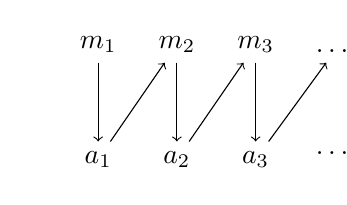
\begin{tikzpicture}
        \node[above] (m1) at (1,1) {$m_1$};
        \node[above] (m2) at (2,1) {$m_2$};
        \node[above] (m3) at (3,1) {$m_3$};
        \node[above] (mdot) at (4,1) {$\dots$};        
        \node[below] (a1) at (1,0) {$a_1$};
        \node[below] (a2) at (2,0) {$a_2$};
        \node[below] (a3) at (3,0) {$a_3$};
        \node[below] (adot) at (4,0) {$\dots$};
        % \draw[->,smooth,postaction={mid arrow=black}] (1,1.2)--(1,0) .. controls (1.2,-0.2) .. (2,1.2);
        \draw[->] (m1) -- (a1);
        \draw[->] (a1) -- (m2);
        \draw[->] (m2) -- (a2);
        \draw[->] (a2) -- (m3);
        \draw[->] (m3) -- (a3);
        \draw[->] (a3) -- (mdot);
    \end{tikzpicture}
    \end{figure}
    Obviously, all elements in $M\cup A$ can be made 1-1 correspondence with $\mathbb{N}$. And $M\sim \mathbb{N}\sim M\cup A$.
    We then consider the case that $M$ is uncountable. Hence $m(M)=c$ and $m(M\cup A) = c$. Both of then have the power of continuum. Therefore they are equivalent.
\end{proof}

\noindent\textit{\textbf{Problem 3.}} Prove that each of the following sets is countable:\\
a) The set of all numbers with two distinct decimal expansions (like $0.5000\dots$ and $0.4999\dots$);\\
b) The set of all rational points in the plane (i.e., points with rational coordinates);\\
c) The set of all rational intervals (i.e., intervals with rational end points);\\
d) The set of all polynomials with rational coefficients.

\begin{proof}
    $    $\newline
    $a)$ Consider the decimal expansion of numbers with 4 and 9. Since this is an infinite-digit-number, one of these numbers must be repeated infinitely after some certain digit. WLOG assume the number ends in all nines.
    \begin{equation*}
        d = 0.d_1d_2d_3\dots\dots d_kd_{k+1}d_{k+2}\dots\dots
    \end{equation*}
    where $d_{k+1} = d_{k+2}=\dots =9 $
    \begin{equation}
    d_i =
    \begin{cases}
        4, \text{for some $i$ if $i\leq k$}\\
        9, \text{for some $i$ if $i\leq k$, and all $i$ if $i>k$}\\
    \end{cases}
    \end{equation}
    Consider the set $D_k=\{d|~d_{k+1}, d_{k+2},\dots are~all~nines\}$, and $Card(D_k)$ is therefore determined by the previous $k$ digits, and there are $2^k$ possibilities. Then the set of interest
    \begin{equation*}
    D(4,9) = \bigcup\limits_{k=1}^{\infty}D_k
    \end{equation*}
    and it is the union of countably many sets, each of which has at most finite elements. Thus $D(4,9)$ is countable. We have hereby proves only one set containing 4 and 9 and ending in all nines. With base 10 number system, we could have the permutation $P_2^9=72$ possibilities including $D(4,9)$. Consider them all could still give us at most countable set.\\
    $b)$ We wish to show that $\mathbb{Q}\times\mathbb{Q}$ is countable. Since $\mathbb{Q}$ is countable, we could list all the elements in ascending order such that:
    \begin{equation*}
    a_1,a_2,a_3,\dots
    \end{equation*}
    and similarly for the y-coordinates we have
    \begin{equation*}
    b_1,b_2,b_3,\dots
    \end{equation*}
    We can thus list all coordinates (or follow the path shown in the graph)(Well, I have to admit that this is rather a poor drawing, but Tikz package are too painful to learn.) 
    \begin{equation*}
    (a_1,b_1),(a_2,b_1),(a_1,b_2),(a_1,b_3),(a_2,b_2),(a_3,b_1),\dots
    \end{equation*}
    \begin{figure}
    \centering
    \begin{tikzpicture}
        \node[below] (1) at (2,2) {$(a_1,b_1)$};
        \node[below] (2) at (4,2) {$(a_2,b_1)$};
        \node[below] (3) at (2,4) {$(a_1,b_2)$};
        \node[below] (4) at (2,6) {$(a_1,b_3)$};
        \node[below] (5) at (4,4) {$(a_2,b_2)$};
        \node[below] (6) at (6,2) {$(a_3,b_1)$};
        \node[below] (7) at (8,2) {$\dots$};
        \draw[->] (1) -- (2);
        \draw[->] (2) -- (3);
        \draw[->] (3) -- (4);
        \draw[->] (4) -- (5);
        \draw[->] (5) -- (6);
        \draw[->] (6) -- (7);
    \end{tikzpicture}
    \end{figure}
    And of course $\mathbb{Q}\times\mathbb{Q}$ is therefore countable.\\
    $c)$ Let $a$ and $b$ be the two end points of the interval, and $a$, $b$ $\in\mathbb{Q}$. Similar to b), we could list them and order them, which shows that all rational intervals are countable.\\
    $d)$ Denote polynomials as
    \begin{equation*}
    p = p_0 + p_1x + p_2x^2 +p_3x^3+ \dots
    \end{equation*}
    where $p_i$ are all rationals. Let the set $P_i=\{p_i|~p_i\in \mathbb{Q}\}$ and clearly it is countable. Let the set
    \begin{equation*}
    P = \bigcup\limits_{i=0}^{\infty}P_i
    \end{equation*}
    which is countably union of countable sets. Thus $P$ is countable.
\end{proof}


\noindent\textit{\textbf{Problem 4.}} A number $\alpha$ is called algebraic if it is a root of a polynomial equation with rational coefficients. Prove that the set of all algebraic numbers is countable.
\begin{proof}
    $     $\newline
    Since there are at most countable number of polynomial equations, each of which has at most $n$ roots, if it is a polynomial of degree $n$. Therefore the roots are countable and therefore is all algebraic numbers.
\end{proof}

\noindent\textit{\textbf{Problem 5.}} Prove the existence of uncountably many \textit{transcendental} numbers, i.e., numbers which are not algebraic.

\begin{proof}
    Since we have countably many algebraic numbers, and there are uncountably in $\mathbb{R}$. It follows that there must be countably transcendental numbers.
\end{proof}

\noindent\textit{\textbf{Problem 6.}} Prove that the set of all real functions 
(more generally, functions taking values in a set containing at least two elements)
defined on a set $M$ is of power greater than the power of $M$. 
In particular, prove that the power of the set of \textit{real} functions
(continuous and discontinuous) defined in the interval$[0,1]$ is greater than $c$.

\begin{proof}
    $    $\newline
\end{proof}

\noindent\textit{\textbf{Problem 7.}} Give an indirect proof of the equivalence of the closed interval $[a,b]$, the open interval $(a,b)$ and the half-open interval $[a,b)$ or $(a,b]$.\\
\textit{Hint}. Use Theorem 7. 
(\textbf{Cantor-Bernstein Theorem}: 
\textit{Given any two sets $A$ and $B$, 
suppose $A$ contains a subset $A_1$ equivalent to $B$, 
while $B$ contains a subset $B_1$ equivalent to $A$. 
Then $A$ and $B$ are equivalent.})
\begin{proof}
    $   $\newline
    I have no idea how to prove this one ``indirectly'', yet having a ``direct'' proof 
    echoing that of ``equivalence of $(0,1)$ and $[0,1]$''. It goes as follows.\\
    Consider a sequence in $(a,b)$,say $(x_n)$. We can form a bijection such that\\
    \begin{figure}[H]
    \centering
    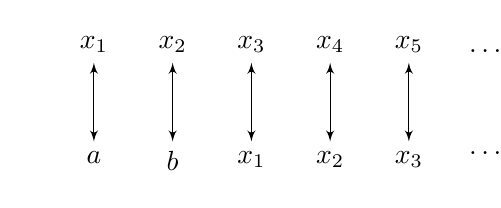
\begin{tikzpicture}
        \node[below] at (0,0) (a) {$a$};
        \node[above] at (0,1) (x1) {$x_1$};
        \draw[latex'-latex'] (a) -- (x1);
        \node[below] at (1,0) (b) {$b$};
        \node[above] at (1,1) (x2) {$x_2$};
        \draw[latex'-latex'] (b) -- (x2);
        \node[below] at (2,0) (x1) {$x_1$};
        \node[above] at (2,1) (x3) {$x_3$};
        \draw[latex'-latex'] (x1) -- (x3);
        \node[below] at (3,0) (x2) {$x_2$};
        \node[above] at (3,1) (x4) {$x_4$};
        \draw[latex'-latex'] (x2) -- (x4);
        \node[below] at (4,0) (x3) {$x_3$};
        \node[above] at (4,1) (x5) {$x_5$};
        \draw[latex'-latex'] (x3) -- (x5);
        \node[below] at (5,0) {$\dots$};
        \node[above] at (5,1) {$\dots$};
    \end{tikzpicture}
    \end{figure}
    In other words, we let $x_{n-2}\longleftrightarrow x_{n}$ , if $n>2$. 
    And we let the rest elements in $(a,b)$ point to itself, i.e., 
    $x\longleftrightarrow x$. Thus, the bijection between $[a,b]$ and $(a,b)$
     is established and we have the equivalence. 
     Similar proof could be used on half-open intervals. \\
     However, I cannot think of an ``indirect'' proof using Cantor-Bernstein Theorem.
\end{proof}

\noindent\textit{\textbf{Problem 8.}} Prove that the union of a finite or countable number of sets 
each of power $c$ is itself of power $c$.
\begin{proof}
    $     $\newline
    
\end{proof}

\noindent\textit{\textbf{Problem 9.}} 
Prove that each of the following sets has the power of the continuum:\\
a) The set of all infinite sequences of positive integers;\\
b) The set of all ordered $n$-tuples of real numbers;\\
c) The set of all infinite sequences of real numbers.
\begin{proof}
    $     $\newline
    a) Suppose that the set of all infinite sequences of positive integers has power
    of $\aleph_0$. Denote this set as $A=\{\alpha_i|~i\in \mathbb{N}\}$.
    Since it is countable, we could list all the elements:
    \begin{equation*}
    \begin{split}
        \alpha_1 &= (a_{11},a_{12},a_{13},\dots)\\
        \alpha_2 &= (a_{21},a_{22},a_{23},\dots)\\
        \dots\\
    \end{split}
    \end{equation*}
    We could therefore have a sequence of integers 
    \begin{equation*}
    d = (d_1,d_2,d_3,\dots)
    \end{equation*}
    such that 
    \begin{equation*}
    d_i = 
    \begin{cases}
    0, a_{ii} \neq 0\\
    2, a_{ii} = 0\\
    \end{cases}
    \end{equation*}
    It is obvious that $d$ is different from any of the element in $A$, 
    and thus we have a contradiction. \\
    b) For any given $n$ numbers to form an ordered tuple, we could have at most $n!$ 
    numbers of results ($P(n,k)=\frac{n!}{(n-k)!}$). 
    But choosing those $n$ elements from uncountable $\mathbb{R}$ has uncountable 
    permutations. Therefore the set is countable.\\
    c) Since we have the result from a), and all positive integers form a subset of $\mathbb{R}$. Therefore set of all infinite sequences of real numbers is also uncountable.
\end{proof}

\noindent\textit{\textbf{Problem 10.}}
Develop a contradiction inherent in the notion of the 
``set of all sets which are not members of themselves.''\\

\noindent \textit{Hint}. Is this set a member of itself?\\

\noindent \textit{Comment}. Thus we will be careful to avoid sets which are ``too big,''
like the ``set of all sets.''
\begin{proof}
    $      $\newline
    This is also known as Russell's paradox. We prove as follows. Define two sets:
    \begin{equation*}
    \begin{split}
        A &= \{ x|~x\in x \}\\
        B &= \{ x|~x\not\in x\}
    \end{split}
    \end{equation*}
    We wish to ask whether $B\in B$. There are only two possibilities: 
    either $B\in B$, or $B\not\in B$. 
    First suppose the former, then we have set $B$ as an element of $B$, and thus
    $B\not\in B$, which is a contradiction.
    Then consider the latter, and we have $B$ not as an element of $B$. 
    Hence $B$ must in $A$, and it follows $B\in B$, which is also a contradiction.
    Therefore there does not exist a ``set of all sets''.
\end{proof}


\section{Ordered Sets and Ordinal Numbers}

\noindent\textit{\textbf{Problem 1.}}
Exhibit both a partial ordering and a simple ordering of the set of all complex numbers.
\begin{proof}
    $    $\newline
    Denote complex numbers as a pair $x=(a,b)$, 
    where $a=Re(x)$ and $b=Im(x)$.
    Define a partial ordering as the following:
    $x_1<x_2$, if $a_1<a_2$.
    We could also define the simple ordering (total order) as:
    $x_1<x_2$, if $a_1<a_2$ or if $a_1=a_2$ and $b_1<b_2$.
\end{proof}

\noindent\textit{\textbf{Problem 2.}}
What is the minimal element of the set of all subsets of a given set $X$, partially ordered by
set inclusion. What is the maximal element?
\begin{proof}
    $   $\newline
    Clearly, the minimal element is $\emptyset$ and the maximal is $X$ itself. 
    Since $\emptyset$ is subset of any set, and $X$ is the only set that contains all
    elements in itself.
\end{proof}

\noindent\textit{\textbf{Problem 3.}}
A partially ordered set $M$ is said to be a \textit{directed set} if, given any two elements
$a, b\in M$, there is an element $c\in M$ such that $a\leq c$, $b\leq c$. 
Are the partially ordered sets in Examples 1-4, Sec. 3.1 all directed sets?
\begin{proof}
    $    $\newline
    a) False. Since $a\leq b$ if and only if $a = b$. Let any two elements
    in $M$, and $x$, $y$ are not necessarily to be equal. If we wish to find a $c$,
    such that $x\leq c$ and $y\leq c$, we must have $x=c=y$. Hence it is
    not a directed set.\\
    b) True. Since $M$ contains all CTS function, there must one function $h(x)$ such that
    given any two other functions $f$ and $g$ in $M$, $f\leq h$ and $g \leq h$
    must hold. Hence it is a directed set.\\
    c) True. Since $\mathcal{M}=\{M_i\}$ is the set of all subsets of $M$, 
    the maximal element must be $M$ itself. Thus, any two sets must be subsets of $M$. 
    It is a directed set.\\
    d) False. Suppose for a contradiction that there exist a $c$ such that any $a$, $b$
    as integers, and $c$ is divisible by both $a$ and $b$. However, there must also exist
    integer $x =  $
\end{proof}

\noindent\textit{\textbf{Problem 4.}}
By the \textit{greatest lower bound} of two elements $a$ and $b$ of a 
partially ordered set $M$, 
we mean an element $c\in M$ such that $c\leq a$, $c\leq b$ and there is
no element $d\in M$ such that $c<d\leq a$, $d\leq b$. Similarly, by the 
\textit{least upper bound} of $a$ and $b$, we mean an element $c\in M$ such that
$a\leq c$, $b\leq c$ and there is no element $d\in M$ such that 
$a\leq d<c$, $b<d$. by a \textit{lattice} is meant a partially ordered
set any two element of which have both a greatest lower bound and a least upper bound.
Prove that the set of all subsets of a given set $X$, 
partially ordered by set inclusion, is a lattice. What is the set-theoretic meaning of 
the greatest lower bound and least upper bound of two elements of this set?
\begin{proof}
    $     $\newline

\end{proof}






\noindent\textit{\textbf{Problem 5.}}
Prove that an order-preserving mapping of one ordered set onto another is automatically
an isomomrphism.
\begin{proof}
    $    $\newline

\end{proof}





\section{System of Sets}

\chapter{Metric Spaces}
\begin{chapquote}{Kolmogorov}
    ``One of the most important operations in mathematical analysis is the taking of limits.''
\end{chapquote}
\section{Basic Concepts}


\section{Convergence. Open and Closed Sets}


\noindent\textit{\textbf{Problem 1.}}\\
\begin{proof}
    $    $\newline
\end{proof}

\noindent\textit{\textbf{Problem 2.}} Prove that every contact point of a set $M$ is either a limit point of $M$ or an isolated point of $M$.\\

\begin{proof}
    $    $\newline
\end{proof}

\noindent\textit{\textbf{Problem 3.}} Prove that if $x_n \to x$, $y_n\to y$ as $n\to \infty$, then $\rho(x_n,y_n)\to \rho(x,y)$.\\
\begin{proof}
    $     $\newline
    Fix $\varepsilon >0$, $\exists~N_1\in \mathbb{N}$, $s.t.~n>N_1$,  $\rho(x_n,x)<\frac{\varepsilon}{2}$. Also $\exists~N_2\in \mathbb{N}$, $s.t.~n>N_2$, $\rho(y_n,y)<\frac{\varepsilon}{2}$. Pick $N=\max(N_1,N_2)$, such that $n>N$, (by 1.a, p.45) we have $|\rho(x_n,y_n)-\rho(x,y)| \leq \rho(x_n,x)+\rho(y_n,y)<\frac{\varepsilon}{2} $.\\
\end{proof}

\noindent\textit{\textbf{Problem 4.}} Let $f$ be a mapping of one metric space $X$ into another metric space $Y$. Prove that $f$ is continuous at a point $x_0$ if and only if the sequence $\{y_n\}=\{f(x_n) \}$ converges to $y=f(x_0)$ whenever the sequence $\{x_n \}$ converges to $x_0$.
\begin{proof}
    $     $\newline
    ``$\Rightarrow$'':\\
    Fix $\varepsilon>0$, $\exists~ \delta>0$, $s.t.~\rho(x_n,x_0)<\delta$ implies $\rho'(f(x_n),f(x_0))$. Hence $(y_n)\to y$, as $n\to\infty$.\\
    ``$\Leftarrow$''\\
    Fix $\varepsilon>0$, $\exists~ \delta>0$,  $\rho'(y_n,y_0)<\varepsilon$ whenever $\rho(x_n,x_0)<\delta$. It implies $\rho'(f(x_n),f(x_0))<\varepsilon$. Therefore, $f$ is continuous at $x_0$.
\end{proof}


\noindent\textit{\textbf{Problem 5.}} Prove that\\
a) The closure of any set $M$ is a closed set;\\
b) $[M]$ is the smallest closed set containing $M$.
\begin{proof}
    $    $\newline
    a) Let $x\in [[M]]$. Fix $\varepsilon>0$, there exist $x_1\in[M]$, $s.t.~x_1\in O_\varepsilon(x)$. Consider $O_{\varepsilon_1}(x_1)$, where $\varepsilon_1=\varepsilon-\rho(x,x_1)$. Since $O_{\varepsilon_1}(x_1)\subset O_\varepsilon(x)$, and there exists $x_2\in O_{\varepsilon_1}(x_1)$ and $x_2\in O_\varepsilon(x)$. Hence $x\in [M]$.\\
    \indent Since we have $x\in [[M]]$ and then it is also in $[M]$. We could have $[[M]]\subset [M]$. With $[M]\subset [[M]]$, we have $[[M]]=[M]$.\\
    b) Suppose $\exists~x \in [M]$, and $x\not\in M$. Therefore $O_\varepsilon(x)\cap M=\emptyset$. Since also $x\in [M]$, $x$ must a contact a point and thus any neighborhood of $x$ contains at least one point of $M$, which is a contradiction. Therefore $[M]$ is the smallest set containing $M$.
\end{proof}

\noindent\textit{\textbf{Problem 6.}} Is the union of infinitely many closed sets necessarily closed? How about the intersection of infinitely many open sets? Give examples.
\begin{proof}
    $    $\newline

\end{proof}

\noindent\textit{\textbf{Problem 7.}} Prove directly the the point $\frac{1}{4}$ belongs to the Cantor set $F$, although it is not an end of any of the open intervals deleted in constructing $F$. (Hint: The point $\frac{1}{4}$ divides the interval $[0,1]$ in the ratio $1:3$. It also divides the interval $[0,\frac{1}{3}]$ left after deleting $(\frac{1}{3},\frac{2}{3})$ in the ratio $3:1$, and so on.)
\begin{proof}
    $    $\\

\end{proof}




\section{Complete Metric Spaces}
\section{Contraction Mappings}






\chapter{Topological Spaces}
\begin{chapquote}{Kolmogorov}
    ``Metric spaces are topological spaces of a rather special (although very important) kind.''
\end{chapquote}
\section{Basic Concepts}
\section{Compactness}
\section{Compactness in Metric Spaces}
\section{Real Functions on Metric and Topological Spaces}

\chapter{Linear Spaces}
\begin{chapquote}{Kolmogorov}
    ``One of the most important concepts in mathematics is that of a linear space, which will play a key role in the rest of this book.''
\end{chapquote}

\section{Basic Concepts}
\section{Convex Sets and Functionals. The Hahn-Banach Theorem}
\section{Normed Linear Spaces}
\section{Euclidean Spaces}


%%%%%%%%%%%%%%%%%%%%%%%%%%%%%%%%%%%%%%%%%%%%%%%%%%%%%%%
% Sample table                                        %
% Source: www1.maths.leeds.ac.uk/latex/TableHelp1.pdf %
%%%%%%%%%%%%%%%%%%%%%%%%%%%%%%%%%%%%%%%%%%%%%%%%%%%%%%%
% \begin{table}[ht]
% \caption{Sample table} % title of Table
% \centering % used for centering table
% \begin{tabular}{c c c c}
% % centered columns (4 columns)
% \hline\hline %inserts double horizontal lines
% S. No. & Column\#1 & Column\#2 & Column\#3 \\ [0.5ex]
% % inserts table
% %heading
% \hline % inserts single horizontal line
% 1 & 50 & 837 & 970 \\
% 2 & 47 & 877 & 230 \\
% 3 & 31 & 25 & 415 \\
% 4 & 35 & 144 & 2356 \\
% 5 & 45 & 300 & 556 \\ [1ex] % [1ex] adds vertical space
% \hline %inserts single line
% \end{tabular}
% \label{table:nonlin} % is used to refer this table in the text
% \end{table}

\end{document}


